
\begin{figure}[!htb]
	\centering

	\begin{tikzpicture}

		\node (Before) at (0,0) {
			% Edge collapse before
			\begin{tikzpicture}[scale=0.5]

				% Vertices


				\coordinate (1) at (10,9);
				\coordinate (2) at (3,7);
				\coordinate (3) at (8,7);
				\coordinate (4) at (3,2);
				\coordinate (5) at (8,6);
				\coordinate (6) at (1,10);
				\coordinate (7) at (9,5);
				\coordinate (8) at (8,4);
				\coordinate (9) at (9,2);
				\coordinate (10) at (1,1);

				% \foreach \i in {1,..., 10}
				% \draw (\i) node {\i};

				\draw[thick] (2) -- (6);
				\draw[thick] (2) -- (4);
				\draw[thick] (2) -- (8);
				\draw[thick] (2) -- (5);
				\draw[thick] (2) -- (3);
				\draw[thick] (8) -- (4);
				\draw[thick] (8) -- (9);
				\draw[thick] (3) -- (5);
				\draw[thick] (8) -- (5);
				\draw[thick] (8) -- (7);
				\draw[thick] (3) -- (1);
				\draw[thick] (5) -- (7);
				\draw[thick] (3) -- (7);
				\draw[thick] (7) -- (1);
				\draw[thick] (9) -- (1);
				\draw[thick] (7) -- (9);
				\draw[thick] (4) -- (9);
				\draw[thick] (10) -- (9);
				\draw[thick] (10) -- (2);
				\draw[thick] (10) -- (6);
				\draw[thick] (10) -- (4);
				\draw[thick] (6) -- (3);
				\draw[thick] (6) -- (1);

				\draw[fill = red] (2) circle (5pt);
				\foreach \i in {3,4,5,6,8,10}
				\draw[fill = blue!50] (\i) circle (3pt);

			\end{tikzpicture}
		};

		\node (After) at (8,0) {
			% Edge collapse before
			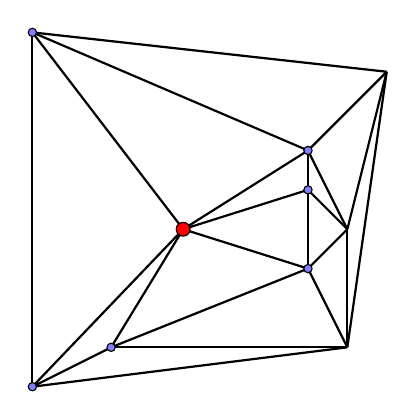
\begin{tikzpicture}[scale=0.5]

				% Vertices


				\coordinate (1) at (10,9);
				\coordinate (2) at (4.83,5);
				\coordinate (3) at (8,7);
				\coordinate (4) at (3,2);
				\coordinate (5) at (8,6);
				\coordinate (6) at (1,10);
				\coordinate (7) at (9,5);
				\coordinate (8) at (8,4);
				\coordinate (9) at (9,2);
				\coordinate (10) at (1,1);


				% \foreach \i in {1,..., 10}
				% \draw (\i) node {\i};

				\draw[thick] (2) -- (6);
				\draw[thick] (2) -- (4);
				\draw[thick] (2) -- (8);
				\draw[thick] (2) -- (5);
				\draw[thick] (2) -- (3);
				\draw[thick] (8) -- (4);
				\draw[thick] (8) -- (9);
				\draw[thick] (3) -- (5);
				\draw[thick] (8) -- (5);
				\draw[thick] (8) -- (7);
				\draw[thick] (3) -- (1);
				\draw[thick] (5) -- (7);
				\draw[thick] (3) -- (7);
				\draw[thick] (7) -- (1);
				\draw[thick] (9) -- (1);
				\draw[thick] (7) -- (9);
				\draw[thick] (4) -- (9);
				\draw[thick] (10) -- (9);
				\draw[thick] (10) -- (2);
				\draw[thick] (10) -- (6);
				\draw[thick] (10) -- (4);
				\draw[thick] (6) -- (3);
				\draw[thick] (6) -- (1);

				\draw[fill = red] (2) circle (5pt);

				\foreach \i in {3,4,5,6,8,10}
				\draw[fill = blue!50] (\i) circle (3pt);


			\end{tikzpicture}
		};

		\draw[->, thick] (Before) -- (After);

	\end{tikzpicture}

	\caption{Example of smoothing a vertex}
	\label{fig:smoothVertex}
\end{figure}
